% Tiny contract
% Teams: arm
% Requirements: REQ-GEN-090, REQ-FUN-100, REQ-DES-140
% Status: done

\subsubsection{End-Effector Design}
\label{subsubsec:end_effector_design}

The rover employs a parallel-jaw gripper mechanism for maintenance operations and sample collection tasks. The design features a dual-linkage symmetric four-bar configuration maintaining parallel finger pad orientation throughout the \qty{105}{\milli\metre} maximum opening range, ensuring uniform pressure distribution and consistent tool center point (TCP) alignment (\autoref{fig:gripper_assembly}).

\begin{figure}[H]
    \centering
    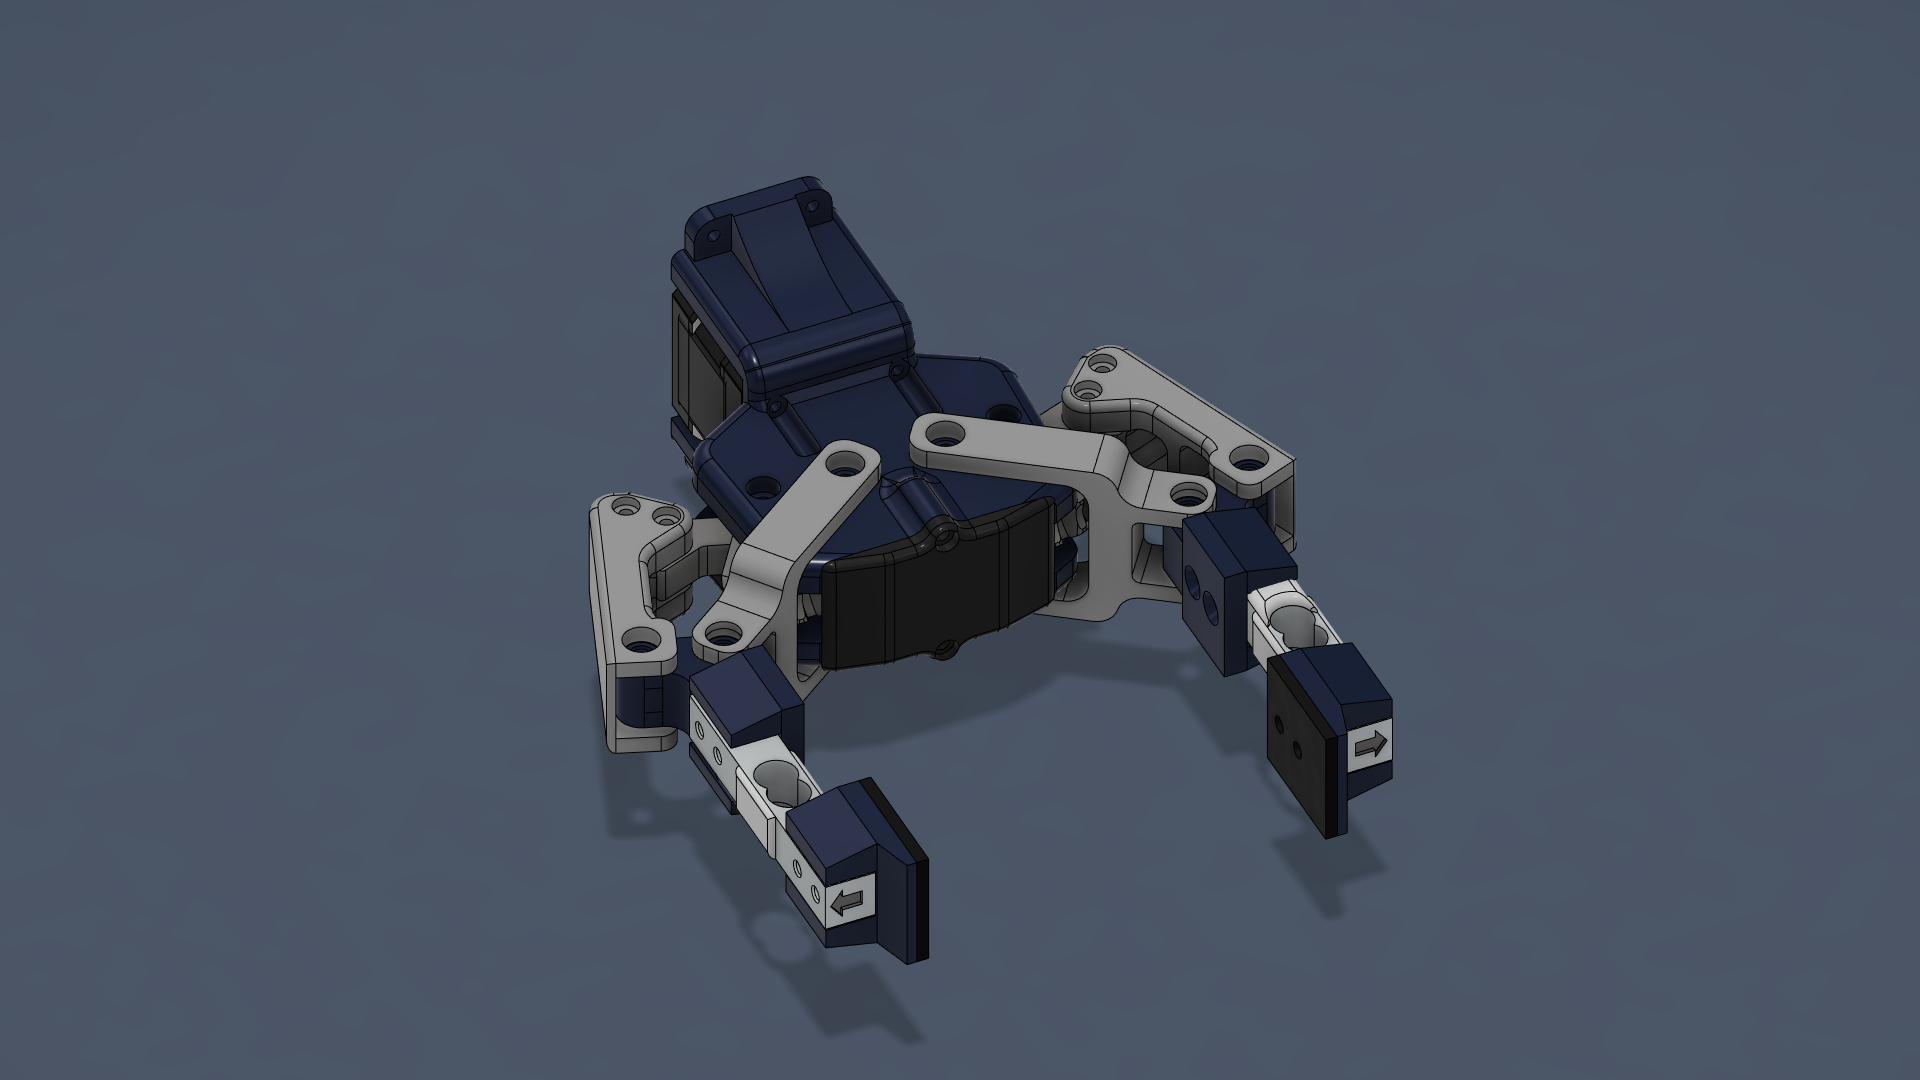
\includegraphics[width=0.7\textwidth]{teams/arm/figures/gripper_assembly.png}
    \caption{Gripper assembly showing dual-linkage mechanism and finger geometry}
    \label{fig:gripper_assembly}
\end{figure}

\paragraph{Kinematic Architecture}
The symmetrically mirrored four-bar linkage arrangement provides mechanical advantage through two aluminum linkages per finger, pinned at discrete pivot points to form a robust mechanical loop. This configuration constrains gripping surfaces to remain parallel during actuation, preventing object rotation and ensuring repeatable force vectors. Symmetric design about both longitudinal and lateral axes maintains grasp center alignment with the TCP for precise manipulation coupled with robotic arm kinematics (\autoref{subsubsec:manipulator_configuration_kinematics}).

\paragraph{Actuation and Force Sensing}
NEMA17 stepper motor actuation provides sufficient torque with inherent overload protection through step-skipping behavior, preventing mechanical damage during constrained motion. Integrated Force-sensitive Hall-effect Dual-Axis (FHDA) load sensors enable closed-loop force control, modulating grip strength based on object compliance to prevent crushing fragile components while ensuring secure retention during manipulation and transport.

\paragraph{Gripper Geometry and Contact Surfaces}
Active gripping surfaces measuring \numproduct{30 x 32}~mm feature molded rubber pads increasing friction while providing mechanical damping. Compliant pads accommodate non-planar geometries and absorb impact forces during tasks such as switch rotation. Fingertip geometry narrows to \qty{10}{\milli\metre} total width for precise engagement with circuit breaker switches (\qtyrange{10}{15}{\milli\metre} width) and small-profile panel targets. Overall dimensions when fully opened are \numproduct{180 x 200 x 80}~mm (W$\times$L$\times$H).

\paragraph{Panel Operation Capabilities}
Parallel-jaw configuration with force feedback enables controlled pressing motions on panel buttons with programmable force profiles. Narrow fingertip geometry permits switch engagement in densely populated control panels. Rubber pad compliance allows rotational manipulation of cylindrical knobs and toggle switches through friction coupling. Combined position control and force sensing support typing, button pressing, and connector insertion/extraction operations on maintenance panels.

\paragraph{Probe Collection}
The gripper accommodates cylindrical aluminum probes (\qty{30}{\milli\metre} diameter, \qty{200}{\milli\metre} height) through its \qty{105}{\milli\metre} maximum jaw opening. Parallel-jaw mechanism distributes gripping forces evenly around probe circumference, preventing structural deformation. Rubber pads provide anti-slip characteristics for secure retention during arm motion and probe extraction from ground insertion points. Force sensing enables adaptive grip pressure accounting for surface conditions and extraction resistance.

\paragraph{Mechanical Interface}
The gripper base features standardized mounting geometry for attachment to the robotic arm's quick-change end-effector mount, enabling rapid tool exchange. Mechanical and electrical interfaces ensure reliable coupling under field conditions with minimal alignment sensitivity.
